\section{Comparação das Curvas Frequência X Temperatura}
\label{sec:ResFreqXTemp}

Com as medidas de frequência durante o aquecimento da câmera térmica da temperatura ambiente até a temperatura alvo foi possível construir as curvas apresentadas nas Figuras \ref{fig:FreqXTempDE21001} e \ref{fig:FreqXTempZedBoard1001}. Cada uma das curvas é construída com os dados de um ciclo de estresse e está relacionada a um tempo de envelhecimento acumulado. Na Tabela \ref{tab:TempoDia} da Seção \ref{sec:MetEnsaios} consta que dia corresponde ao ciclo de cada uma das curvas.

Na Figura \ref{fig:FreqXTempDE21001} 
se vê que as curvas estão próximas e que não há uma sequência entre elas com relação ao tempo de envelhecimento, visto que a curva de 24 horas (vermelha) é a posicionada mais abaixo.

\begin{figure}[H]
    \centering
    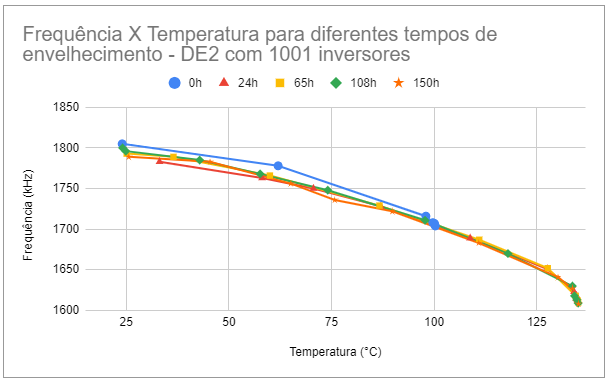
\includegraphics[scale=0.75]{figures/Resultados/FreqXTempDE21001}
    \caption{Curva Frequência por Temperatura do oscilador com 1001 inversores da placa DE2. Fonte: O Autor}
    \label{fig:FreqXTempDE21001}
\end{figure}

No entanto, na Figura \ref{fig:FreqXTempZedBoard1001} é observado que as curvas estão ordenadas em relação ao tempo de envelhecimento, sendo deslocadas para baixo a cada sido. Ou seja, é possível verificar que, de forma geral, a frequência em qualquer temperatura foi diminuindo com o estresse térmico.

\begin{figure}[H]
    \centering
    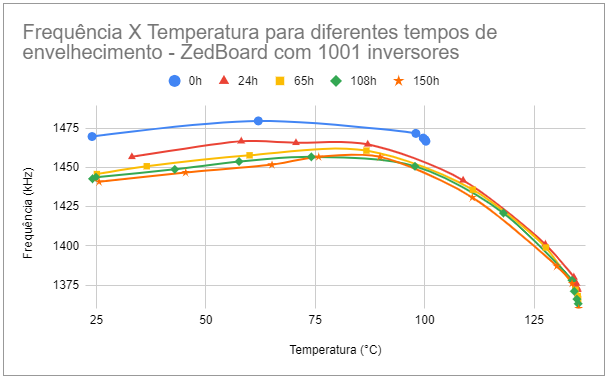
\includegraphics[scale=0.75]{figures/Resultados/FreqXTempZedBoard1001}
    \caption{Curva Frequência por Temperatura do oscilador com 1001 inversores da placa ZedBoard. Fonte: O Autor}
    \label{fig:FreqXTempZedBoard1001}
\end{figure}

Essas duas figuras corroboram com o discutido na Seção \ref{sec:ResTAmb} de que os osciladores da ZedBoard apresentaram uma degradação consideravelmente maior que os osciladores da DE2.
